\documentclass[12pt,a4paper]{article}

\usepackage{amsmath} % у преамбулі

\usepackage{caption}
\captionsetup[table]{name=Таблиця}  % замість "Табл." буде "Таблиця"

\usepackage{listings}
\usepackage{xcolor}

\lstset{
    language=Python,           % або інша мова програмування
    basicstyle=\ttfamily\small,
    numbers=left,              % нумерація рядків зліва
    numberstyle=\tiny\color{gray},
    stepnumber=1,
    numbersep=5pt,
    frame=single,              % рамка навколо коду
    backgroundcolor=\color{white},
    keywordstyle=\color{blue}\bfseries,
    commentstyle=\color{green!50!black},
    stringstyle=\color{red},
    breaklines=true,           % перенос рядків
    captionpos=b,              % підпис під лістингом
    showstringspaces=false,
    tabsize=4
}


\renewcommand{\thetable}{№\arabic{table}}

\usepackage[utf8]{inputenc}
\usepackage[T2A]{fontenc}
\usepackage[ukrainian]{babel}
\usepackage{graphicx} % <-- Для роботи з \includegraphics
\usepackage{geometry}
\geometry{
    left=2cm,
    right=2cm,
    top=2cm,
    bottom=2cm
}

\begin{document}

    \begin{titlepage}

        \thispagestyle{empty}
        \begin{center}
        \large
        Національний технічний університет України\\
        «Київський політехнічний інститут імені Ігоря Сікорського»\\[1em]
        Факультет інформатики та обчислювальної техніки\\
        Кафедра загальної фізики
        \end{center}

        \vfill

        \begin{center}
        \textbf{\Large Фізика}\\[2em]
        \textbf{\Large Лабораторна робота №ФПЕ-10}\\
        «Дослідження згасаючих коливань у коливальному контурі» 
        \end{center}

        \vfill

        \begin{flushright}
        Виконав: студент 1 курсу ФІОТ, гр. ІО-41\\
        \textit{Давидчук А. М.}\\
        Залікова книжка № 4106\\[1em]
        Перевірив: \textit{Колган В.\,В.}
        \end{flushright}

        \vfill

        \begin{center}
        Київ -- 2025
        \end{center}

    \end{titlepage}

    \setlength{\parindent}{0pt}

    % main document

    \textbf{\underline{Тема:}} «Дослідження згасаючих коливань у коливальному контурі».

    \vspace{1em} % вручну задаєте відступ

    \textbf{\underline{Мета:}} визначення параметрів та характеристик реального коливального контуру.

    \vspace{1em} % вручну задаєте відступ

    \textbf{\underline{Прилади та устаткування:}} Блок-схема експериментальної установки (рис. 3.1): ГЗ-111 --- генератор звукових сигналів ГЗ-111; С1-76 --- осцилограф С1-76;
    ФПЭ-10/11 --- касета з контуром ФПЕ-10/11; ПІ-ФПЭ-09 --- перетворювач імпульсів; Дж --- джерело живлення; МО --- магазин опорів.

    \begin{figure}[h!]

        \setcounter{figure}{0}                  % скидаємо лічильник фігур
        \renewcommand{\thefigure}{3.\arabic{figure}} % робимо "3.1", "3.2" і т.д.

        \centering
        % Підставляєте потрібний шлях та розмір зображення:
        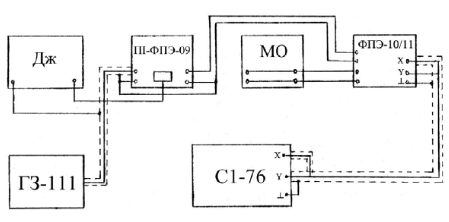
\includegraphics[width=0.5\textwidth]{3.1.png}
        % Підпис (зазвичай під малюнком):
        \caption{Загальна схема досліду}
        % Мітка для посилань у тексті (\ref{fig:...})
        \label{fig1:schema}
    \end{figure}

    %%%%%%%%%%%%%%%%%%%%%%%%%%%%%%%%%%%Теоретичні відомості%%%%%%%%%%%%%%%%%%%%%%%%%%%%%%%%%%%

    \begin{center}
        \textbf{\Large Теоретичні відомості}
    \end{center}

    \vspace{1em} % вручну задаєте відступ

    \setlength{\parindent}{1.5em}

    Реальний коливальний контур складається з послідовно з’єднаних конденсатора $C$, котушки індуктивності $L$
    і резистора $R$. Якщо зарядити конденсатор від батареї Б до напруги $U$ (рис. 3.2), а потім від’єднати батарею
    за допомогою ключа $K$, то конденсатор почне розряджатися через котушку і у контурі виникнуть електромагнітні коливання.

    \begin{figure}[h!]

        \renewcommand{\thefigure}{3.\arabic{figure}} % робимо "3.1", "3.2" і т.д.

        \centering
        % Підставляєте потрібний шлях та розмір зображення:
        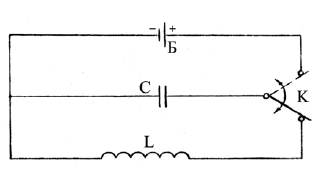
\includegraphics[width=0.5\textwidth]{3.2.png}
        % Підпис (зазвичай під малюнком):
        \caption{Загальна схема досліду}
        % Мітка для посилань у тексті (\ref{fig:...})
        \label{fig2:schema}

    \end{figure}

    Спочатку розглянемо випадок, коли опір контуру $R$ = 0.

    Після замикання контуру в ньому виникне розрядний струм $I$, який не відразу набуває максимального значення.
    Плавна зміна сили струму в колі зумовлена появою в котушці ЕРС самоіндукції, яка за правилом Ленца перешкоджає зміні струму,
    тобто гальмує розряд конденсатора. Як тільки заряд конденсатора стане рівним нулю, сила струму в контурі досягне максимуму.
    З цього моменту сила струму в колі починає зменшуватися, не змінюючи свого напрямку.
    В цьому випадку ЕРС самоіндукції підтримує струм, який викликав її появу.
    Ця ж ЕРС призводить до перезаряджання конденсатора, після чого процес повторюється, однак з іншим напрямом струму.
    Надалі ці процеси повторюються, тобто виникають коливання.

    Час, протягом якого в коливальному контурі відбувається один повний цикл змін і контур повертається в початковий стан, називають періодом електричного коливання.

    Якщо активний опір в контурі дорівнює 0, то коливання в контурі можуть продовжуватися нескінченно довго.
    Такі коливання, які відбуваються внаслідок процесів у самому коливальному контурі без зовнішніх впливів і втрат енергії,
    називають власними електричними коливаннями. Вони є незагасаючими.

    У початковий момент, коли конденсатор був заряджений, у ньому була накопичена енергія

    \begin{center}
        $\displaystyle W_e = \frac{CU^2}{2}.$
    \end{center}

    Під час розрядки енергія електричного поля конденсатора перетворюється в енергію магнітного поля котушки і,
    коли конденсатор повністю розряджений, енергія магнітного поля досягає максимального значення:

    \begin{center}
        $\displaystyle W_m = \frac{LI_0^2}{2}$,
    \end{center}

    де $I_0$ --- амплітуда сили струму в контурі. Під час перезаряджання конденсатора енергія магнітного поля знову перетворюється на енергію електричного поля.
    За умови $R$ = 0 у контурі відбуваються незагасаючі електромагнітні коливання.

    Усі без винятку провідники за звичайних умов мають відмінний від нуля опір, тому частина енергії при
    коливаннях витрачається на їх нагрівання, тобто перетворюється на теплову і втрачається.
    В наслідок цього амплітуда електромагнітних коливань в контурі зменшується
    відбувається загасання коливань (рис. 3.3).

    \begin{figure}[h!]

        \renewcommand{\thefigure}{3.\arabic{figure}} % робимо "3.1", "3.2" і т.д.

        \centering
        % Підставляєте потрібний шлях та розмір зображення:
        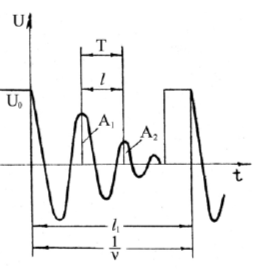
\includegraphics[width=0.3\textwidth]{3.3.png}
        % Підпис (зазвичай під малюнком):
        \caption{Графік згасаючих коливань}
        % Мітка для посилань у тексті (\ref{fig:...})
        \label{fig3:schema}

    \end{figure}

    При достатньо великому опорі контуру або малій індуктивності коливання у ньому взагалі не виникають,
    а відбувається так званий аперіодичний розряд конденсатора.

    Заряд конденсатора і сила струму у котушці коливального контуру постійно змінюються
    за значенням і напрямом. Вважатимемо, що в момент часу $t$ заряд на обкладинках
    конденсатора $q$, напруга на ньому $\displaystyle U_C = \frac{q}{C}$, а сила струму у колі
    змінюється зі швидкістю $\displaystyle \frac{dI}{dt}$. У котушці індуктивності виникає ЕРС самоіндукції

    \begin{equation}
        \mathcal{E}_L = -L\frac{dI}{dt}.
        \tag{3.1}
    \end{equation}

    Відповідно до другого правила Кірхгофа для коливального контуру, опір якого дорівнює нулю, можна записати

    \begin{equation}
        U + \mathcal{E}_L = IR,
        \tag{3.2}
    \end{equation}

    де

    \begin{equation}
        I = -\frac{dq}{dt}.
        \tag{3.3}
    \end{equation}

    (струм тече в додатному напрямку при зменшенні заряду конденсатора).

    Оскільки $q = CU$, то з урахуванням (3.1) та (3.2) отримаємо:

    \begin{center}
        $\displaystyle I = -C \frac{dU}{dt}$,
    \end{center}

    \begin{center}
        $\displaystyle \mathcal{E}_L = LC \frac{d^2U}{dt^2}$.
    \end{center}

    Підставивши останній вираз в (3.2), матимемо:

    \begin{equation}
        \frac{d^2U}{dt^2} + \frac{R}{L} \frac{dU}{dt} + \frac{U}{LC} = 0.
        \tag{3.4}
    \end{equation}

    Як відомо, диференціальне рівняння (3.4) є рівнянням загасаючих електричних коливань.
    Розв’язком цього рівняння є функція

    \begin{equation}
        U = U_0e^{-\beta t} \cos(\omega t + \alpha).
        \tag{3.5}
    \end{equation}

    де $\beta$ --- коефіцієнт загасання,

    \begin{equation}
        \beta = \frac{R}{2L},
        \tag{3.6}
    \end{equation}

    де $\omega$ --- циклічна частота загасаючих коливань,

    \begin{equation}
        \omega = \sqrt{\frac{1}{LC} - \left( \frac{R}{2L}\right)^2}.
        \tag{3.7а}
    \end{equation}

    При цьому

    \begin{equation}
        \omega = \frac{2\pi}{T} \text{  та  } T = \frac{2\pi}{\sqrt{\dfrac{1}{LC} - \left( \dfrac{R}{2L}\right)^2}}.
        \tag{3.7б}
    \end{equation}

    Якщо (3.2) записати у вигляді

    \begin{center}
        $\displaystyle \frac{q}{C} + IR = -\frac{dI}{dt}$
    \end{center}

    та взяти похідну за часом, то отримаємо рівняння подібне до рівняння (3.4):

    \begin{center}
        $\displaystyle \frac{d^2I}{dt^2} + \frac{R}{L} \frac{dI}{dt} + \frac{I}{LC} = 0$.
    \end{center}

    Отже, сила струму $I$ в контурі також здійснює загасаючі коливання (щоправда, початкова фаза цих коливань буде іншою),
    для яких значення $\beta$ й $\omega$ визначаються формулами (3.6), (3.7а) та (3.7б).

    З (3.7а) та (3.7б) видно, що в коливальному контурі можливі загасаючі коливання лише у випадку,
    якщо $\displaystyle \frac{1}{LC} > \left( \frac{R}{2L}\right)^2$ (частота та період є дійсними величинами)
    або $\displaystyle R < 2\sqrt{\frac{L}{C}}$, то частота і період – уявні величини, коливань немає і відбувається
    аперіодичний розряд конденсатора.

    Опір

    \begin{equation}
        R_K = 2\sqrt{\frac{L}{C}}
        \tag{3.8}
    \end{equation}

    називають критичним.

    Щоб характеризувати загасаючі коливання, окрім коефіцієнта загасання $\beta$,
    використовується ще логарифмічний декремент (лат. dekrement --- зменшення) загасання.

    Логарифмічним декрементом загасання називається натуральний логарифм
    відношення значень напруги, розділених інтервалом часу,
    який дорівнює періоду коливань $T$,

    \begin{equation}
        \lambda = \ln \frac{A_1}{A_2} = \ln \frac{A(t)}{A(t+T)},
        \tag{3.9}
    \end{equation}

    або

    \begin{center}
        $\displaystyle \lambda \approx 2,3\cdot \lg \frac{A_1}{A_2}$.
    \end{center}

    Підставивши в (3.9) значення $A(t) = U_0e^{-\beta t}$ та $A(t+T) = U_0e^{-\beta (t+T)}$, отримаємо

    \begin{equation}
        \lambda = \beta T,
        \tag{3.10}
    \end{equation}

    або згідно (3.6)

    \begin{equation}
        \lambda = \frac{R}{2L}T.
        \tag{3.10а}
    \end{equation}

    У деяких випадках зручно вивчати коливний процес у системі координат $I$ та $U$,
    тобто відкладати на осі абсцис значення сили струму в контурі,
    а на осі ординат -- напругу на конденсаторі у той же момент часу.
    Площина $IU$ має назву площини станів, або фазової площини, а крива,
    яка зображає залежність напруги від струму, називається фазовою кривою (див. рис. 3.4).

    \begin{figure}[h!]

        \renewcommand{\thefigure}{3.\arabic{figure}} % робимо "3.1", "3.2" і т.д.

        \centering
        % Підставляєте потрібний шлях та розмір зображення:
        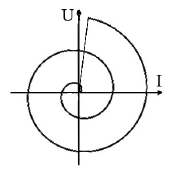
\includegraphics[width=0.3\textwidth]{3.4.png}
        % Підпис (зазвичай під малюнком):
        \caption{Фазова крива}
        % Мітка для посилань у тексті (\ref{fig:...})
        \label{fig4:schema}

    \end{figure}

    Знайдемо фазову криву для контуру, опір якого $R = 0$. цьому випадку
    $\displaystyle \beta = \frac{R}{2L} = 0$ і тоді з (3.5), (3.7а) та (3.7б) отримуємо

    \begin{equation}
        \omega = \sqrt{\frac{1}{LC}},\text{ } T = 2\pi \sqrt{LC},
        \tag{3.11}
    \end{equation}

    \begin{equation}
        \left\{
        \begin{aligned}
            U &= U_0 \cos \omega t \\
            I &= -C \frac{dU}{dt} = U_0 \omega C \sin \omega t
        \end{aligned}
        \right.
        \tag{3.12}
    \end{equation}

    Рівняння (3.11), (3.12) описують незагасаючі коливання.
    Виключивши з них час $t$, отримаємо рівняння фазової кривої (рівняння еліпса):

    \begin{center}
        $\displaystyle \frac{U^2}{U_0^2} - \frac{I^2}{U_0^2 \omega^2 C^2} = 1$.
    \end{center}

    Еліпс можна отримати у результаті накладання двох взаємно перпендикулярних
    гармонічних коливань (3.12), із зсувом фаз у чверть періоду.

    У контурі, опір якого $R>0$, відбуваються загасаючі коливання напруги (3.5) та струму:
    \begin{center}
        $
        \left\{
        \begin{aligned}
            U &= U_0 e^{-\beta t} \cos \omega t \\
            I &= -C \frac{dU}{dt} = U_0C e^{-\beta t} (\beta \cos \omega t + \omega \sin \omega t)
        \end{aligned}
        \right.
        $
    \end{center}

    У цьому випадку амплітуди напруги та сили струму у контурі безперервно
    спадають і фазова крива буде незамкненою (рис.3.4).

    У даній роботі для отримання коливань у контурі використовується касета
    ФПЕ-10/11 з контуром, зображеним на рис. 3.5.

    \begin{figure}[h!]

        \renewcommand{\thefigure}{3.\arabic{figure}} % робимо "3.1", "3.2" і т.д.

        \centering
        % Підставляєте потрібний шлях та розмір зображення:
        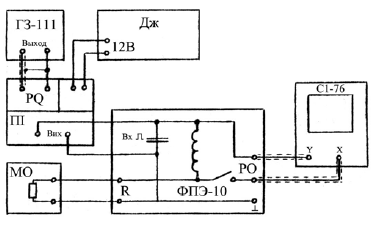
\includegraphics[width=0.5\textwidth]{3.5.png}
        % Підпис (зазвичай під малюнком):
        \caption{Схема експериментальної установки}
        % Мітка для посилань у тексті (\ref{fig:...})
        \label{fig5:schema}

    \end{figure}

    Загасаючі коливання, які відбуваються у контурі, спостерігаються на екрані
    осцилографа С1-76. Цикл зарядки та розрядки конденсатора продовжується
    протягом часу $T = \dfrac{1}{v}$, де $v$ – частота, яка задається звуковим
    генератором ГЗ-111. На екрані осцилографа йому відповідає відрізок $l_1$.
    Це дозволяє визначити період $T$ загасаючих коливань,
    якому на рис. 3.3 відповідає відрізок l. З пропорції $\dfrac{l}{T} = l_1v$ отримаємо

    \begin{equation}
        T = \frac{l}{l_1v}.
        \tag{3.14}
    \end{equation}

    %%%%%%%%%%%%%%%%%%%%%%%%%%%%%%%%%%%Теоретичні відомості%%%%%%%%%%%%%%%%%%%%%%%%%%%%%%%%%%%

    \newpage

    \begin{center}
        \textbf{\Large Практична частина}
    \end{center}

    \vspace{1em} % вручну задаєте відступ

    \setlength{\parindent}{0pt}

    \textbf{Порядок виконання завдання №1:}

    \vspace{1em} % вручну задаєте відступ

    \setlength{\parindent}{1.5em}

    1. Включив лабораторний стенд і переконався, що він готовий до роботи (загорілася лампочка «Сеть»).

    2. Запустив генератор сигналів ГЗ-111 та виставив частоту $\nu = 250$ Гц.

    3. Включив джерело живлення та активував перетворювач імпульсів ПІ-ФПЕ-09, вибравши відповідні налаштування (клавіша «П» і «Скважность грубо»).

    4. На магазині опорів послідовно встановлював значення $R_m = $ 100, 200, 300, 400, 500, 600 Ом.

    5. За допомогою осцилографа С1-76 отримував стабільну картину загасаючих коливань.

    6. Виміряв довжини відрізків $l$ і $l_1$ на екрані осцилографа та розрахував період коливань $T$ за формулою (3.14).

    7. Виміряв значення амплітуд коливань ($A_1$, $A_2$, $A_3$) та розрахував логарифмічний декремент $\lambda$ за формулою (3.9), а також коефіцієнт загасання $\beta$ за формулою (3.10) для кожного зі значень $R_m$. Всі результати заніс у таблицю №1.

    8. Побудував графік залежності $\lambda$ від опору магазину опорів $R_m$, визначивши внутрішній опір котушки $r_k$ за допомогою екстраполяції графіка $\lambda(R_m)$ до 0. Відовідно, обчислишви значення $r_k$, я обчислив значення повного
    опору $R$ для кожного значення опору $R_m$: $R = R_m + r_k$.

    9. Розрахував середні значення індуктивності $L$ з формули (3.10а) і ємності $C$ контуру з формули (3.11) періоду для мого досліду. Тобто

    \begin{center}
        $\displaystyle L = \frac{R}{2\lambda} T$ \text{  та  } $\displaystyle C = \left( \frac{T}{2\pi} \right)^2 \cdot \frac{1}{L}$.
    \end{center}

    10. Визначив критичний опір $R_{cr}$ за формулою (3.15), за якого спостерігається аперіодичний розряд конденсатора, і перевірив відповідність цього значення розрахунковим співвідношенням.

    \begin{equation}
        R_{cr} = 2 \sqrt{\frac{L}{C}}.
        \tag{3.15}
    \end{equation}

    \vspace{1em} % вручну задаєте відступ

    \setlength{\parindent}{0pt}

    \textbf{Порядок виконання завдання №2:}

    \vspace{1em} % вручну задаєте відступ

    \setlength{\parindent}{1.5em}

    1. Перевів осцилограф у режим фазової діаграми.
    
    2. Встановлював фазові криві в центр екрана та вимірював значення вертикальної напруги $U$ та горизонтальної $U$ екрана осцилографа з кроком в одни період.

    3. За формулою (3.9) обчислював логарифмічний декремент $\lambda$ як за вертикальною напругою (вже обчислені дані в таблиці №1), так і за силою струму, яку можна знайти з відношення $U = IR_m$.

    4. Результати всіх вимірювань заносив до таблиці №2.

    5. Оцінив похибку вимірювань логарифмічного декременту для $U$ та $I$ за формулою

    \begin{center}
        $\displaystyle \Delta \lambda_X = \sqrt{\frac{\Delta X_1^2}{X_1} + \frac{\Delta X_2^2}{X_2}}, \quad X = 
        \begin{cases}
        U\\
        I
        \end{cases}$
    \end{center}

    \vspace{1em} % вручну задаєте відступ
    \setlength{\parindent}{0pt}

    \textbf{Всі вимірювання проводив у симуляторі лабораторної роботи ФПЕ-10 (FPE10)!}

    \newpage

    \textbf{\large Завдання №1:}

    \vspace{1em} % вручну задаєте відступ

    Під час вимірювань величин $l$ та $l_1$, я отримав такі значення:

    \vspace{1em} % вручну задаєте відступ

    $l = 4 \cdot 10^{-3}$ с, $l_1 = 0,4$ с.

    \vspace{1em} % вручну задаєте відступ

    Звідси $T$ = $\displaystyle \frac{l}{l_1 \nu} = \frac{0,4}{4 \cdot 10^{-3} \cdot 250} = \frac{0,4}{1} = 0,4$ с.

    \vspace{1em} % вручну задаєте відступ
    \setlength{\parindent}{1.5em}

    Далі змінюватиму $R_m$, вимірюватиму величини $A_1$, $A_2$, $A_3$ та за наявних даних, обчислю всі значення таблиці за допомогою Python коду (лістинг 1.1).
    Значення $r_k$ я знайду, побудувавши графік $\lambda(R_m)$ та знайшовши точку перетину з віссю абсцис (див. рис. 3.6).

    \begin{table}[h!]
        \centering
        \renewcommand{\arraystretch}{1.2} % відстань між рядками
        \begin{tabular}{|c|c|c|c|c|c|c|c|c|c|}
            \hline
            $R_m$, Ом & $A_1$, В & $A_2$, В & $A_3$, В & $\lambda$ & $\beta$, c$^{-1}$ & $L$, Гн & $C$, мкФ & $r_k$, Ом & $R$, Ом \\[3pt]
            \hline
            100 & 5,4547 & 4,5516 & 3,8292 & 0,2359 & 0,5897 & 138,2 & 29,32 & 63,0058 & 163 \\[3pt]
            200 & 4,8768 & 3,6485 & 2,7093 & 0,3919 & 0,9797 & 134,2 & 30,19 & & 263 \\[3pt]
            300 & 4,3710 & 2,8899 & 1,8785 & 0,5630 & 1,4080 & 129,0 & 31,43 & & 363 \\[3pt]
            400 & 3,9014 & 2,2758 & 1,3366 & 0,7141 & 1,7850 & 129,7 & 31,26 & & 463 \\[3pt]
            500 & 3,4679 & 1,8423 & 0,9392 & 0,8709 & 2,1770 & 129,3 & 31,34 & & 563 \\[3pt]
            600 & 3,0706 & 1,4450 & 0,6864 & 0,9988 & 2,4970 & 132,8 & 30,53 & & 663 \\[3pt]
            \hline
        \end{tabular}
        \caption{Результати розрахунку $\lambda$, $\beta$, $R$, $L$, $C$ коливального контуру.}
    \end{table}

    \begin{figure}[h!]

        \renewcommand{\thefigure}{3.\arabic{figure}} % робимо "3.1", "3.2" і т.д.

        \centering
        % Підставляєте потрібний шлях та розмір зображення:
        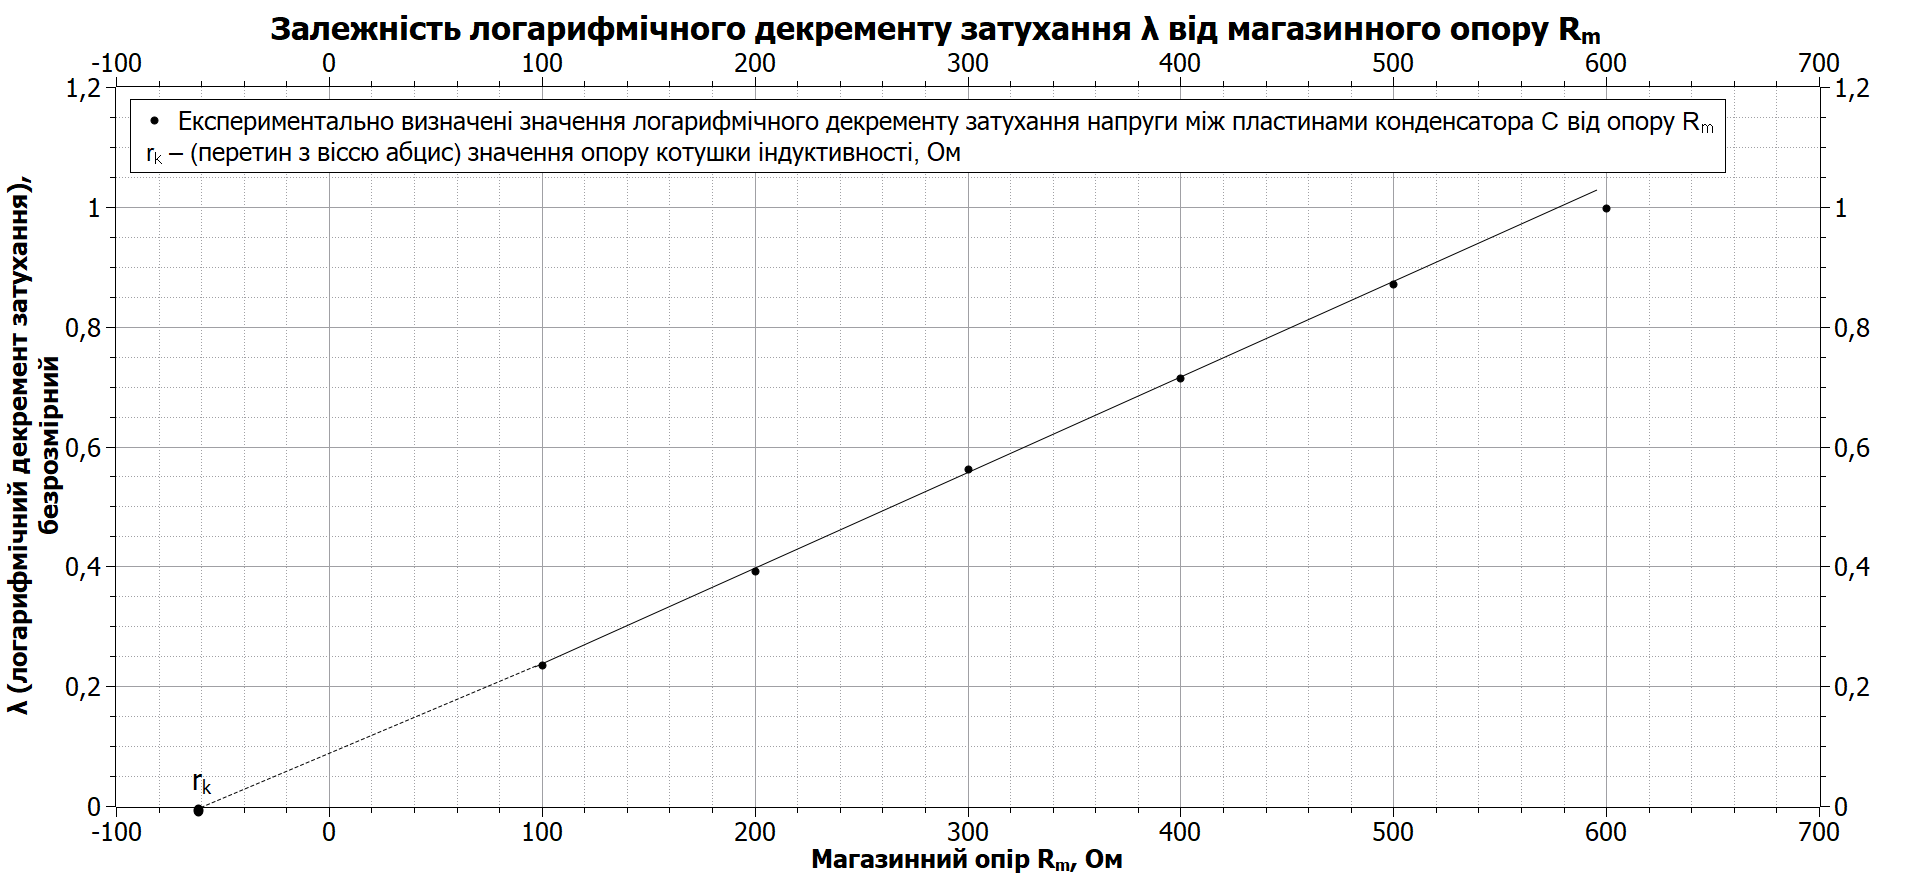
\includegraphics[width=1.00\textwidth]{graph.png}
        % Підпис (зазвичай під малюнком):
        \caption{Графік $\lambda(R_m)$}
        % Мітка для посилань у тексті (\ref{fig:...})
        \label{graph:schema}

    \end{figure}

    Також додатково було пораховано середнє значення індуктивності $L$, ємності $C$ контуру, як середнє арифметичне значення в таблиці №1 та відносно них
    $R_{cr}$ за формулою (3.15):

    \vspace{1em} % вручну задаєте відступ
    \setlength{\parindent}{0pt}

    ⟨$L$⟩ = 132,2 Гн; ⟨$C$⟩ = 29,32 мкФ;   $R_{cr}$ = 4088,5 Ом.

    \newpage

    Результат виконання програми з лістингу 1.1:

    \begin{figure}[ht]
        \centering
        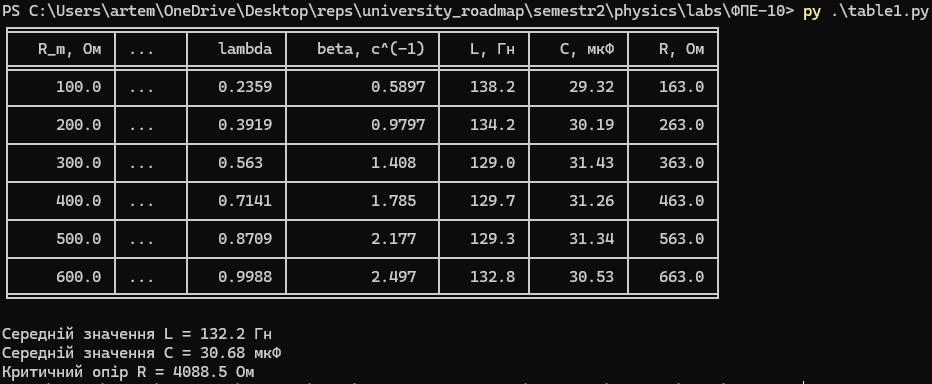
\includegraphics[width=1\textwidth]{table1_results.png}
    \end{figure}

    \vspace{1em} % вручну задаєте відступ

    \textbf{\large Обчислення похибок для завдання №1:}

    \vspace{1em} % вручну задаєте відступ
    \setlength{\parindent}{1.5em}

    В ході виконання завдання №1, використовувались такі величини: експериментально визначені значення (пряме вимірювання) $R_m$, $l$, $l_1$, $A_i$, де $i = \overline{1, 3}$ та $r_k$;
    теретично визначені значення (непрямі вимірювання) $T$, $\lambda$, $\beta$, $R$, $L$, $C$ та $R_{cr}$. Почнемо розгляд з експериментально визначених величин.

    Величини $R_m$ та $r_k$ які являються опорами, тобто теоретично їх можна розглядати, як опір 2 резисторів. Зазвичай, резистори,
    які використовуються в лабораторній роботі мають клас точності 5\%, тобто відносна похибка для резистора $R$ та $r_k \approx$ 5\% = 0,05. Абсолютну похибку
    вираховують шляхом множення номінального значення резистора на його відносну похибку. З резистором $r_k$ все дуже прозоро, так як цей резистор статичний, прийнамні, не враховується його зміна через зміну температури.
    І його абсолютна похибка буде $\Delta r_k = r_k \cdot 0,05 = 63,0058 \cdot 0,05 \approx 3,15$ Ом. Ось ситуація з опором $R_m$ складніша: ми використовували його із різними значеннями.
    В такому випадку, я знайду середнє арифметичне значення $R_m$ в діапазоні змін, тобто від 100 до 600, а потім отриманий результат помножу на відносну похибку 5\%.

    \vspace{1em} % вручну задаєте відступ
    \setlength{\parindent}{0pt}

    $\displaystyle \Delta R_m \approx \frac{R_{m_i}}{6} \cdot 0,05, i = \overline{1, 6} \approx \frac{100 + 200 + 300 + 400 + 500 + 600}{6} \cdot 0,05 = \frac{2100}{6} \cdot 0,05 = 17,5$ Ом.

    \setlength{\parindent}{1.5em}

    Щодо величин $l_1$ та $l$ --- вони були визначені за допомогою поділок на екрані осцилографа. Ціна однієї поділки в режимі залежності $U = f(t)$ на осі абцис $\Delta t$ = $10^{-3}$ с. Так як даних про похибку
    самого зображення на екрані осилографа у нас немає, візьмемо середнє поширене значення в 3\%. Аболютну похибку для $l_1$ та $l$ можна обчислити за формулою

    \begin{center}
        $\displaystyle \Delta l = \sqrt{(\Delta T_k)^2 + (\Delta T_c)^2}$,
    \end{center}

    де $\Delta T_k$ --- похибка калібрування осцилографа, $\Delta T_k = T \cdot 0,03$, а $\Delta T_c$ --- похибка вимірювання, $\Delta T_c = \Delta t \cdot k$, де $k = 0,2$ --- похибка відліку для екрану осцилографа.
    Тут за $T$ ми приймаємо значення $l$ та $l_1$. Відносні похибки можна обчислити за формулою $\displaystyle \varepsilon = \frac{\Delta l}{l}$.

    Для $l$ матимемо:

    \vspace{1em} % вручну задаєте відступ

    $\displaystyle \Delta T_k = 4 \cdot 10^{-3} \cdot 0,03 = 12 \cdot 10^{-5}$ c, $\displaystyle \Delta T_c = 10^{-3} \cdot 0,2 = 2 \cdot 10^{-4}$ c.

    $\displaystyle \Delta l = \sqrt{\left( 12 \cdot 10^{-5}\right)^2 + \left(2 \cdot 10^{-4}\right)^2} = \sqrt{144 \cdot 10^{-10} + 4 \cdot 10^{-8}} \approx 23,32 \cdot 10^{-5}$ с.

    $\displaystyle \varepsilon_l = \frac{23,32 \cdot 10^{-5}}{4 \cdot 10^{-3}} \approx 0,0533 \approx 5,33\%$.

    \vspace{1em} % вручну задаєте відступ

    Для $l_1$ матимемо:

    \vspace{1em} % вручну задаєте відступ

    $\displaystyle \Delta T_k = 0,4 \cdot 0,03 = 12 \cdot 10^{-3}$ c, $\displaystyle \Delta T_c = 10^{-3} \cdot 0,2 = 2 \cdot 10^{-4}$ c.

    $\displaystyle \Delta l_1 = \sqrt{\left( 12 \cdot 10^{-3}\right)^2 + \left(2 \cdot 10^{-4}\right)^2} = \sqrt{144 \cdot 10^{-6} + 4 \cdot 10^{-8}} \approx 12 \cdot 10^{-3}$ с.

    $\displaystyle \varepsilon_{l_1} = \frac{12 \cdot 10^{-3}}{0,4} \approx 0,03 \approx 3\%$.

    \vspace{1em} % вручну задаєте відступ

    Щодо величин $A$, то вони також були виміряні за допомогою екрану осцилографа, а це значить, що формули для обчислення похибок залишуться такими ж самими, але проблема в тому, що
    даних $A$ є купа, а це значить, що потрібно визначати середнє значення, а саме середньоквадратичне відхилення абсолютних та відносних їх похибок, а разом із ним, потрібно буде помножити на коефіцієнт
    Стьюдента, який при довірчому коефіцієнту $\alpha = 0,9$ та кількістю вимірювань $i = 18$, буде дорівнювати $t_{(0,9; 18)} = 1,73$.

    Так як даних багато, я викорстаю Python код (Лістинг 3.2) для розрахунку похибок, і не тільки для $A$ (див. далі). Результат виконання програми показує, що $\Delta A \approx 0,0108$ В, $\varepsilon_{A} \approx 2,3358$ \%.

    Щодо теоретичних величин, то для обчислення похибок для непрямих вимірів використовуватимемо Гаусові формули для поширення похибок:

    \[
        \Delta y \;=\;
        \sqrt{
        \left(
            \frac{\partial f}{\partial a}\Bigg|_{\substack{a=\langle a\rangle \\ b=\langle b\rangle \\ \dots}}
        \right)^{2} S_{(a)}^{2}
        \;+\;
        \left(
            \frac{\partial f}{\partial b}\Bigg|_{\substack{a=\langle a\rangle \\ b=\langle b\rangle \\ \dots}}
        \right)^{2} S_{(b)}^{2}
        \;+\;\dots
        }
    \]

    \[
        \varepsilon_y \;=\;
        \sqrt{
        \left(
            \frac{\partial \ln f}{\partial a}\Bigg|_{\substack{a=\langle a\rangle \\ b=\langle b\rangle \\ \dots}}
        \right)^{2} S_{(a)}^{2}
        \;+\;
        \left(
            \frac{\partial \ln f}{\partial b}\Bigg|_{\substack{a=\langle a\rangle \\ b=\langle b\rangle \\ \dots}}
        \right)^{2} S_{(b)}^{2}
        \;+\;\dots
        } \cdot 100 \%
    \]

    \vspace{1em} % вручну задаєте відступ

    Почнемо з величини $T$ --- ця функція залежить від 3 змінних: $l_1$, $l$ та $\nu$. Відповідно,

    \begin{center}

        $\displaystyle T = \frac{l}{l_1 \nu}$; $\displaystyle \frac{\partial T}{\partial l_1} = -\frac{l}{l_1^2 \nu}$; $\displaystyle \frac{\partial T}{\partial l} = \frac{1}{l_1 \nu}$; $\displaystyle \frac{\partial T}{\partial \nu} = -\frac{l}{l_1 \nu^2}$;
        $\displaystyle \frac{\partial \ln T}{\partial l_1} = -\frac{1}{l_1}$; $\displaystyle \frac{\partial \ln T}{\partial l} = \frac{1}{l}$; $\displaystyle \frac{\partial \ln T}{\partial \nu} = -\frac{1}{\nu}$;

    \end{center}

    \begin{center}

        $\displaystyle \Delta T = \sqrt{\left( \frac{\text{⟨}l\text{⟩}}{\text{⟨}l_1^2\text{⟩} \text{⟨}\nu\text{⟩}} S_{l_1} \right)^2 + \left( \frac{S_l}{\text{⟨}l_1\text{⟩} \text{⟨}\nu\text{⟩}} \right)^2 + \left(\frac{\text{⟨}l\text{⟩}}{\text{⟨}l_1\text{⟩} \text{⟨}\nu\text{⟩}^2} S_{\nu}  \right)^2}$,

    \end{center}

    \begin{center}

        $\displaystyle \varepsilon_T = \sqrt{\left( \frac{S_{l_1}}{\text{⟨}l_1\text{⟩}} \right)^2 + \left( \frac{S_l}{\text{⟨}l\text{⟩}} \right)^2 + \left( \frac{S_{\nu }}{\text{⟨}\nu \text{⟩}} \right)^2} \cdot 100 \%$,

    \end{center}

    де $\text{⟨}l_1\text{⟩} = l_1 = 0,4$ c, $\text{⟨}l\text{⟩} = l = 0,5$ с, $\text{⟨}\nu\text{⟩} = \nu = 250$ Гц. Значення $S_{l_1}$ та $S_l$ були попередньо визначені, та дорівнюють $S_{l_1} = S_l = T_c = 2 \cdot 10^{-4}$ с.
    Значення для $S_{\nu}$ можна визначити, що генератор звукових сигналів ГЗ-111 має клас точності 0,1\% в середньому, тобто $\varepsilon_{\nu} = 0,1$ \%, а це значить, що $\Delta \nu = S_{\nu} = \nu \cdot 0,001 = 0,25$ Гц.
    Вiдповiдно, за результатами програми з Лiстингу 3.2, $\Delta T \approx 2 \cdot 10^{-6}$ с, $\varepsilon_T \approx 5$ \%.

    Розглянемо величину $\lambda$, яка залежить за формулою від 2 змінних: $A_i$ та $A_{i+1}$, але насправді, ми обчислювали її 3 рази, для різних значень $A_i$, а потім знаходили середнє арифметичне.
    Тобто на значення $\lambda$ впливали 3 змінні: $A_i$, $A_{i+1}$ та $A_{i+2}$. Тобто в нашій роботі, ця функція залежить від 3 змінних.
    Значить формула для $\lambda$ це 

    \begin{center}
        $\displaystyle \lambda_i = \frac{\ln \frac{A_i}{A_{i+1}} + \ln \frac{A_i}{A_{i+2}} + \ln \frac{A_{i+1}}{A_{i+2}}}{3}$,
    \end{center}

    звідси, якщо ми розпишемо частку підлогарифмічних функцій як різницю логарифмів, ми спростимо функцію до 2 змінних:

    \begin{center}
        $\displaystyle \lambda_i = \frac{2}{3} \ln \frac{A_i}{A_{i+2}}$,
    \end{center}

    звідси

    \begin{center}
        $\displaystyle \frac{\partial \lambda_i}{\partial A_i} = \frac{2}{3A_i}$; $\displaystyle \frac{\partial \lambda_i}{\partial A_{i+2}} = -\frac{2}{3A_{i+2}}$;
    \end{center}

    \begin{center}
        $\displaystyle \frac{\partial \ln \lambda_i}{\partial A_i} = \frac{1}{\ln \frac{A_i}{A_{i+2}}}$; $\displaystyle \frac{\partial \ln \lambda_i}{\partial A_{i+2}} = -\frac{1}{\ln \frac{A_i}{A_{i+2}}}$;
    \end{center}

    Відповідно, вирази для обчислення похибок для $\lambda$:

    \begin{center}
        $\displaystyle \Delta \lambda = \sqrt{\left( \frac{2}{3\text{⟨}A_i\text{⟩}} S_{A_i} \right)^2 + \left( \frac{2}{3\text{⟨}A_{i+2}\text{⟩}} S_{A_{i+2}}\right)^2}$,
    \end{center}

    \begin{center}
        $\displaystyle \varepsilon_{\lambda} = \sqrt{\left( \frac{S_{A_i}}{\ln \frac{\text{⟨}A_i\text{⟩}}{\text{⟨}A_{i+2}\text{⟩}}}\right)^2 + \left( \frac{S_{A_{i+2}}}{\ln \frac{\text{⟨}A_i\text{⟩}}{\text{⟨}A_{i+2}\text{⟩}}} \right)^2} \cdot 100 \% =
        \frac{\sqrt{S_{A_i}^2 + S_{A_{i+2}}^2}}{\ln \frac{\text{⟨}A_i\text{⟩}}{\text{⟨}A_{i+2}\text{⟩}}} \cdot 100 \% = \frac{\sqrt{S_{A_i}^2 + S_{A_{i+2}}^2}}{\ln \text{⟨}A_i\text{⟩} - \ln \text{⟨}A_{i+2}\text{⟩}} \cdot 100 \%$
    \end{center}

    де

    \begin{center}
        ⟨$\displaystyle A_i$⟩ = $\displaystyle \frac{5,4547 + 4,8768 + 4,3710 + 3,9014 + 3,4679 + 3,0706}{6} \approx 4,1904$ В,
    \end{center}

    \begin{center}
        ⟨$\displaystyle A_{i+2}$⟩ = $\displaystyle \frac{3,8292 + 2,7093 + 1,8785 + 1,3366 + 0,9392 + 0,6864}{6} \approx 1,8965$ В.
    \end{center}

    Ціна однієї поділки на екрані осцилографа по вертикалі дорівнює $\Delta u = $2,26 В --- звідси похибка вимірювання дорівнює $\Delta u \cdot 0,02 = 2,26 \cdot 0,2 = 0,452$ В.
    Відповідно, за результатами програми з Лістингу 3.2, $S_{A_i} = 0,003$ В, $S_{A_{i+2}} = 0,0028$ В, а, відповідно $\Delta \lambda \approx 0,0091$, $\varepsilon_{\lambda} \approx 0,52$ \%.

    Щодо $\beta$: функція залежить від 2 змінних: $\lambda$ та $T$.

    Відповідно

    \begin{center}
        $\displaystyle \beta = \frac{\lambda}{T}$; $\displaystyle \frac{\partial \beta}{\partial \lambda} = \frac{1}{T}$; $\displaystyle \frac{\partial \beta}{\partial T} = -\frac{\lambda}{T^2}$;
        $\displaystyle \frac{\partial \ln \beta}{\partial \lambda} = \frac{1}{\lambda}$; $\displaystyle \frac{\partial \ln \beta}{\partial T} = -\frac{1}{T}$;
    \end{center}

    \begin{center}
        $\displaystyle \Delta \beta = \sqrt{\left( \frac{S_{\lambda}}{\text{⟨}T\text{⟩}} \right)^2 + \left( \frac{\text{⟨}\lambda\text{⟩}}{\text{⟨}T\text{⟩}^2} S_T \right)^2} =
        \frac{1}{\text{⟨}T\text{⟩}^2} \sqrt{\left(\text{⟨}T\text{⟩} S_{\lambda}\right)^2 + \left(\text{⟨}\lambda\text{⟩} S_T\right)^2}$
    \end{center}

    \begin{center}
        $\displaystyle \varepsilon_{\beta} = \sqrt{\left( \frac{S_{\lambda}}{\text{⟨}\lambda\text{⟩} }\right)^2 +
        \left(\frac{S_T}{\text{⟨}T\text{⟩}} \right)^2} \cdot 100 \%$
    \end{center}

    де

    \begin{center}
        ⟨$\lambda$⟩ = $\displaystyle \frac{0,2359 + 0,3919 + 0,5630 + 0,7141 + 0,8709 + 0,9988}{6} \approx 0,6039$, ⟨$T$⟩ = $T$ = 0,4 с,
    \end{center}

    а за попередніми розрахунками $S_{\lambda} = 0,0091$, $S_T = 2 \cdot 10^{-6}$ c. Вiдповiдно, за результатами
    програми з Лiстингу 3.2 $\Delta \beta \approx 0,0228 \text{ с}^{-1}$, $\varepsilon_{\beta} \approx 1,51$ \%.

    Щодо функції $R$, то вона залежить від 2 змінних: $R_m$ та $r_k$. Відповідно

    \begin{center}
        $\displaystyle R = R_m + r_k$; $\displaystyle \frac{\partial R}{\partial R_m} = 1$; $\displaystyle \frac{\partial R}{\partial r_k} = 1$;
        $\displaystyle \frac{\partial \ln R}{\partial R_m} = \frac{\partial \ln R}{\partial r_k} = \frac{1}{R}$;
    \end{center}

    \begin{center}
        $\displaystyle \Delta R = \sqrt{S_{R_m}^2 + S_{r_k}^2}$;
        $\displaystyle \varepsilon_R = \sqrt{\left( \frac{S_{R_m}}{\text{⟨}R_m\text{⟩}} \right)^2 + \left( \frac{S_{r_k}}{\text{⟨}r_k\text{⟩}} \right)^2} \cdot 100 \%$;
    \end{center}

    де

    \begin{center}

        $\displaystyle \text{⟨}R_m\text{⟩} = \frac{100+200+300+400+500+600}{6} = 350$ Ом, $\text{⟨}R_k\text{⟩} = r_k = 63,0058$ Ом,

    \end{center}

    а за попередніми розрахунками $S_{R_m} = \Delta R_m = 17,5$ Ом, $S_{r_k} = \Delta r_k = 3,15$ Ом. Вiдповiдно, за результатами
    програми з Лiстингу 3.2 $\Delta R \approx 17,7812$ Ом, $\varepsilon_R \approx 7,07$ \%.

    Тепер розглянемо функцію індуктивності $L$, яка залежить від 3 змінних: $R$, $\lambda$ та $T$. Відповідно

    \begin{center}

        $\displaystyle L = \frac{R}{2\lambda}T$; $\displaystyle \frac{\partial L}{\partial R} = \frac{T}{2\lambda}$; $\displaystyle \frac{\partial L}{\partial \lambda} = -\frac{R}{2\lambda^2}T$; $\displaystyle \frac{\partial L}{\partial T} = \frac{R}{2\lambda}$;
        $\displaystyle \frac{\partial \ln L}{\partial R} = \frac{1}{R}$; $\displaystyle \frac{\partial \ln L}{\partial \lambda} = -\frac{1}{\lambda}$; $\displaystyle \frac{\partial \ln L}{\partial T} = \frac{1}{T}$;

    \end{center}

    \begin{center}

        $\displaystyle \Delta L = \sqrt{\left( \frac{\text{⟨}T\text{⟩}}{2\text{⟨}\lambda\text{⟩}} S_{R} \right)^2 + \left( \frac{\text{⟨}R\text{⟩}}{2\text{⟨}\lambda^2\text{⟩}} \text{⟨}T\text{⟩} S_{R}\right)^2 + \left( \frac{\text{⟨}R\text{⟩}}{2\text{⟨}\lambda\text{⟩}} S_{\lambda} \right)^2}$;
        $\displaystyle \varepsilon_L = \sqrt{\left( \frac{S_{R}}{\text{⟨}R\text{⟩}} \right)^2 + \left( \frac{S_{\lambda}}{\text{⟨}\lambda\text{⟩}} \right)^2 + \left( \frac{S_{T}}{\text{⟨}T\text{⟩}} \right)^2} \cdot 100 \%$;

    \end{center}

    де $\text{⟨}T\text{⟩}$ = 0,4 с, $\text{⟨}\lambda\text{⟩}$ = 0,6039 с, $\text{⟨}R\text{⟩}$ = 350 Ом, а також за попередніми розрахунками $S_R = \Delta R = 17,7812$ Ом, $S_T = \Delta T = 2 \cdot 10^{-6}$ c,
    $S_{\lambda} = \Delta \lambda = 0,0091$. Вiдповiдно, за результатами програми з Лiстингу 3.2 $\Delta L \approx 7,3311$ Гн, $\varepsilon_L \approx 5,2991$ \%.

    Тепер можемо переходити до функції ємності конденсатора $C$, яка залежить від 2 змінних: $L$ та $T$. Відповідно

    \begin{center}
        $\displaystyle C = \left( \frac{T}{2\pi} \right)^2 \cdot \frac{1}{L}$; $\displaystyle \frac{\partial C}{\partial L} = -\left( \frac{T}{2\pi L} \right)^2$; $\displaystyle \frac{\partial C}{\partial T} = \frac{T}{2\pi L^2}$;
        $\displaystyle \frac{\partial \ln C}{\partial L} = -\frac{1}{L}$; $\displaystyle \frac{\partial \ln C}{\partial T} = \frac{2}{T}$;
    \end{center}

    \begin{center}
        $\displaystyle \Delta C = \sqrt{\left( \left( \frac{\text{⟨}T\text{⟩}}{2\pi\text{⟨}L\text{⟩}} \right)^2 S_{L} \right)^2 + \left( \frac{\text{⟨}T\text{⟩}}{2\pi\text{⟨}L^2\text{⟩}} S_T \right)^2}$;
        $\displaystyle \varepsilon_C = \sqrt{\left( \frac{S_{L}}{\text{⟨}L\text{⟩}} \right)^2 + \left( \frac{S_{T}}{\text{⟨}T\text{⟩}} \right)^2} \cdot 100 \%$;
    \end{center}

    де

    ⟨$L$⟩ = $\displaystyle \frac{138,2 + 134,2 + 129 + 129,7 + 129,3 + 132,8}{6} \approx 132,2$ Гн, ⟨$T$⟩ = $T$ = 0,4 с, а значення для $S_L$ та $S_T$ були попередньо визначені, тобто $S_{L} = \Delta L = 7,3311$ Гн,
    $S_T = \Delta T = 2 \cdot 10^{-6}$ c. Вiдповiдно, за результатами програми з Лiстингу 3.2 $\Delta C \approx 4,2502$ мкФ, $\varepsilon_C \approx 5,5455$ \%.

    Функція $R_{cr}$ залежить від 2 змінних: $C$ та $L$. Відповідно

    \begin{center}
        $\displaystyle R_{cr} = 2 \sqrt{\frac{L}{C}}$; $\displaystyle \frac{\partial R_{cr}}{\partial C} = -\sqrt{\frac{L}{C^3}}$; $\displaystyle \frac{\partial R_{cr}}{\partial L} = \frac{1}{\sqrt{LC}}$;
        $\displaystyle \frac{\partial \ln R_{cr}}{\partial C} = -\frac{1}{2C}$; $\displaystyle \frac{\partial \ln R_{cr}}{\partial L} = \frac{1}{2L}$;
    \end{center}

    \begin{center}
    
        $\displaystyle \Delta R_{cr} = \sqrt{\left( \sqrt{\frac{\text{⟨}L\text{⟩}}{\text{⟨}C\text{⟩}^3}} S_C\right)^2 + \left( \frac{S_L}{\sqrt{\text{⟨}L\text{⟩}\text{⟨}C\text{⟩}}} \right)^2}$;
        $\displaystyle \varepsilon_{R_{cr}} = \sqrt{\left( \frac{S_C}{2\text{⟨}C\text{⟩}} \right)^2 + \left( \frac{S_L}{2\text{⟨}L\text{⟩}} \right)^2} \cdot 100 \%$;

    \end{center}

    \newpage

    де ⟨$C$⟩ = $\displaystyle \frac{29,32 + 30,19 + 31,43 + 31,26 + 31,34 + 30,43}{6} \cdot 10^{-6} = 30,55 \cdot 10^{-6}$ Ф, ⟨$L$⟩ $\approx 132,2$ Гн, $S_C = \Delta C = 4,2502 \cdot 10^{-6}$ Ф, $S_L = \Delta L = 7,3311$ Гн.
    Відповідно до результатів програми з Лістингу 3.2 $\Delta R_{cr} \approx ...$ Ом, $\varepsilon_{R_{cr}} \approx ... \%$.

    %\setlength{\parindent}{1.5em}

\end{document}